\chapter{General Purpose \texttt{GPU} - \texttt{GP-GPU}}

Le \texttt{GPU} (Graphics Processing Units) e le \texttt{CPU} (Central Processing Units) presentano differenze significative nella loro architettura e nel design, riflettendo le loro finalità di utilizzo orientate rispettivamente al throughput e alla latenza.

\begin{tabular}[b]{c}
  
\begin{tikzpicture}[scale=0.4]
    \dram      { 0  ,-2.5}
    \cpucache  { 0  , 0}
    \cpucontrol{ 0  ,4.4}
    \cpualu    { 8.6,4.4}
    \cpualu    {12.8,4.4}
    \cpualu    { 8.6,6.55}
    \cpualu    {12.8,6.55}
    \node[font=\sffamily\bfseries] at (8.45,-3.5) {CPU};
  \end{tikzpicture}\\
  Central Processing Unit (\texttt{CPU})
  \end{tabular}
  \qquad
  \begin{tabular}[b]{c}
  
\begin{tikzpicture}[scale=0.4]
    \dram{0,-2.5}
    \foreach \i in {0,...,7}
      \gpucontrol{0,1.1*\i+0.5}
      \gpucache{0,1.1*\i}
      \foreach \j in {1,...,16}
        \gpualu{\j,1.1*\i};
    \node[font=\sffamily\bfseries] at (8.45,-3.5) {GPU};
  \end{tikzpicture}\\
  Graphical Processing Unit (\texttt{GPU})
\end{tabular}

\section{Architettura delle \texttt{CPU}}
Le \texttt{CPU} sono progettate con un'orientamento alla riduzione della latenza:
\begin{itemize}
    \item \textbf{Grandi cache}: Per convertire gli accessi alla memoria a lunga latenza in accessi alla cache a breve latenza.
    \item \textbf{Controllo sofisticato}: Includono la previsione dei branch per ridurre la latenza dei branch e il forwarding dei dati per ridurre la latenza dei dati.
    \item \textbf{\texttt{ALU} potenti}: Unità di elaborazione aritmetica progettate per ridurre la latenza delle operazioni.
\end{itemize}

\section{Architettura delle \texttt{GPU}}
Al contrario, le \texttt{GPU} sono progettate per massimizzare il throughput:
\begin{itemize}
    \item \textbf{Piccole cache}: Ottimizzate per aumentare il throughput della memoria.
    \item \textbf{Controllo semplice}: Non dispongono di previsione dei branch né di forwarding dei dati.
    \item \textbf{\texttt{ALU} efficienti dal punto di vista energetico}: Numerose \texttt{ALU}, caratterizzate da lunghe latenze ma fortemente pipeline per un alto throughput.
    \item \textbf{Necessità di un numero massivo di thread}: Per tollerare le latenze grazie all'alto numero di thread in esecuzione.
\end{itemize}

\section{Differenze nella Gestione della Memoria}
Entrambe le architetture utilizzano la \texttt{DRAM} come memoria principale,
ma si differenziano significativamente nelle loro strategie di gestione della
cache e nel controllo delle unità di elaborazione, riflettendo i loro obiettivi
di progettazione di bassa latenza per le \texttt{CPU} e alto throughput per
le \texttt{GPU}.

\subsection{Comparazione delle Prestazioni tra \texttt{CPU} e \texttt{GPU}}

\paragraph{\texttt{CPU} per Codice Sequenziale}
Le \texttt{CPU} (Central Processing Units) sono ottimizzate per l'esecuzione
di codice sequenziale dove la latenza è un fattore critico. Grazie alla loro
architettura complessa, che include una gestione avanzata della cache e unità
di controllo sofisticate, le \texttt{CPU} possono eseguire codice sequenziale
molto più rapidamente rispetto alle \texttt{GPU}. Questo le rende particolarmente
adatte per applicazioni che richiedono un elevato grado di interattività o tempi
di risposta rapidi, poiché possono essere fino a 10 volte o più veloci delle
\texttt{GPU} nell'esecuzione di codice sequenziale.

\paragraph{\texttt{GPU} per Codice Parallelo}
Al contrario, le \texttt{GPU} (Graphics Processing Units) sono progettate
per massimizzare il throughput, specialmente utile in applicazioni che
beneficiano dell'elaborazione parallela. Con migliaia di core più piccoli,
le \texttt{GPU} gestiscono efficacemente compiti paralleli, distribuendo
il lavoro su molti core per elaborare grandi quantità di dati simultaneamente.
Questo le rende ideali per computazione scientifica, elaborazione di immagini
e applicazioni di machine learning, dove possono superare le \texttt{CPU} di
un fattore di 10 volte o più in termini di velocità.

\paragraph{Scelta dell'Hardware Adatto}
La scelta tra \texttt{CPU} e \texttt{GPU} deve essere fatta in base alla
natura del carico di lavoro. Mentre le \texttt{CPU} sono preferibili per
operazioni che richiedono decisioni rapide e poca parallelizzazione, le
\texttt{GPU} sono la scelta migliore per lavori che possono essere facilmente
suddivisi in compiti più piccoli e gestiti in parallelo. La decisione dovrebbe
quindi basarsi sull'analisi del carico di lavoro specifico e delle esigenze di
prestazione richieste.

\section{Introduzione a \texttt{CUDA C}}
\texttt{CUDA C} è un'estensione del linguaggio di programmazione \texttt{C} che
consente di scrivere codice per le \texttt{GPU} di \texttt{NVIDIA}. Questo
linguaggio permette di sfruttare la potenza di calcolo delle \texttt{GPU} per
eseguire operazioni parallele su grandi quantità di dati. \texttt{CUDA C} è
progettato per essere simile a \texttt{C}, ma include alcune estensioni e
funzionalità specifiche per la programmazione parallela su \texttt{GPU}.



\subsection{Interazione tra \texttt{CPU} e \texttt{GPU}}

In un'applicazione \texttt{CUDA}, la \texttt{CPU} funge da \textbf{host} e
la \texttt{GPU} come \textbf{device}. Il programma inizia la sua esecuzione
sulla \texttt{CPU} con la funzione \texttt{main} e, al richiamo di una
funzione \textbf{kernel}, trasferisce l'esecuzione sulla \texttt{GPU}.
Questo permette di sfruttare l'elaborazione parallela per poi ritornare
alla \texttt{CPU} una volta completate le operazioni sulla \texttt{GPU}.

\subsection{Esecuzione del \texttt{Kernel CUDA}}

Un \textbf{Cuda kernel} è eseguito da una griglia (\textit{array}) di thread.
Tutti i thread in questa griglia eseguono lo stesso codice scritto nel
kernel. È fondamentale identificare ogni thread mediante un indice unico
per garantire che ciascuno esegua il codice in modo appropriatamente ``diverso".

\subsection{Struttura della Grid e Blocchi di Thread}

Le thread non sono aggregate in un unico gruppo all'interno della griglia,
ma sono organizzate in \textbf{blocchi}. Quindi, abbiamo una griglia
composta da blocchi di thread. Questa strutturazione è essenziale
per facilitare la comunicazione e la sincronizzazione delle thread
all'interno dello stesso blocco, grazie alla presenza di una memoria
condivisa. Le thread in blocchi diversi, tuttavia, hanno capacità
limitate di cooperazione diretta, rendendo la memoria condivisa
all'interno dei blocchi uno strumento cruciale per l'efficienza
del parallelismo.


\begin{figure}[H]
  \centering
  \begin{tikzpicture}[font=\small]

    \matrix[label={[anchor=south west, name=gl]north west:Grid}] (OneGrid) [column sep=1mm, row sep=1mm]
    {\pic{block}; & \pic{block}; & \pic{block}; \\
    \pic {block}; & \pic (Ref) {block}; & \pic{block}; \\
    };
    \begin{scope}[on background layer]
    \node[fit=(OneGrid) (gl), inner sep=0pt, fill=green, draw=gray] (Grid) {};
    \end{scope}
    
    
    \matrix[label={[name=ml]Block(1,1)}, below=2cm of Grid] (OneBlock) [column sep=-\pgflinewidth, row sep=\pgflinewidth]
    {\pic{thread}; & \pic{thread}; & \pic{thread}; & \pic{thread}; \\
    \pic{thread}; & \pic{thread}; & \pic{thread}; & \pic{thread}; \\
    \pic{thread}; & \pic{thread}; & \pic{thread}; & \pic{thread}; \\
    };
    \begin{scope}[on background layer]
    \node[fit=(OneBlock) (ml), inner sep=0pt, fill=yellow, draw=gray] (Block) {};
    \end{scope}
    
    \draw[dashed] (RefBl.north west) -- (Block.north west);
    \draw[dashed] (RefBl.north east) -- (Block.north east);
    
    \end{tikzpicture}
\end{figure}

\section{Identificare le Thread in un Kernel \texttt{CUDA}}
La programmazione in \texttt{CUDA} permette di identificare le thread
in uno spazio che può avere fino a tre dimensioni, rappresentate come
\((x, y, z)\). Questo consente agli sviluppatori di adattare l'assegnazione
delle thread alla struttura dei dati che devono essere elaborati.

\subsection{Array Monodimensionale}

Consideriamo il caso di un array di \(128\) elementi. In una struttura
monodimensionale, è naturale assegnare a ogni blocco \(128\) thread,
utilizzando solo la dimensione \(x\) per identificarle. In questo modo,
ogni thread può essere associato direttamente a un elemento dell'array,
e l'indice \texttt{x} del thread corrisponde all'indice dell'elemento
nell'array:

\begin{lstlisting}
    index = threadIdx.x; 
    array[index] = ...; // Operazioni su ogni elemento dell'array
\end{lstlisting}

\subsection{Matrice Bidimensionale}

Per una matrice di dimensioni \(20 \times 20\) \textit{$400$ elementi},
possiamo utilizzare una configurazione bidimensionale per i blocchi
e le thread. Assegnando \(400\) thread per blocco, ogni thread può
essere identificato tramite le coordinate \((x, y)\), permettendo
di mappare direttamente le coordinate della matrice:

\begin{lstlisting}
    row = threadIdx.y;
    col = threadIdx.x; 
    matrix[row][col] = ...; // Operazioni sulla matrice
\end{lstlisting}

\subsection{Strutture Tridimensionali}

Nel caso di strutture tridimensionali, come un cubo, possiamo estendere
ulteriormente questo concetto. I thread e i blocchi possono essere
configurati in tre dimensioni \((x, y, z)\), ognuna corrispondente
a una dimensione del cubo. Questo permette di indirizzare un elemento
specifico dentro un array tridimensionale in modo diretto:

\begin{lstlisting}
    row = threadIdx.y;
    col = threadIdx.x; 
    depth = threadIdx.z;
    cube[row][col][depth] = ...; // Operazioni sul cubo
\end{lstlisting}

\begin{figure}[H]
  \centering 
  \begin{tikzpicture}[line join=round, line cap=round,%
    x={(1 cm,0 cm)}, y={(0 cm,-1cm)}, z={(0.5 cm,0.5 cm)}]
    \foreach\i in {0,1}
    {%
    \cube{(5*\i,0,0)}{4}{yellow}{0}{1}{}{0}
    \foreach\c in {1,0} \foreach\b in {1,0} \foreach\a in {0,1,2} 
    {%
    \cube{(5*\i+1.2*\a-1.2,1.2*\b-0.6,1.2*\c-0.6)}{1}{orange}{1}{0}{$\a,\b,\c$}{0.5+3*\b}
    }
    \cube{(5*\i,0,0)}{4}{none}{1}{0}{Block $\i$}{2}
    }
  \end{tikzpicture}
\end{figure}
\section{Somma tra Vettori in \texttt{CUDA}}
Per esemplificare il concetto di programmazione parallela in \texttt{CUDA},
consideriamo il problema della somma tra due vettori. Questo problema
è particolarmente adatto alla programmazione parallela, poiché ogni
elemento del vettore può essere sommato indipendentemente dagli altri.

\begin{figure}[H]
  \centering
  \begin{tikzpicture}[
    node distance = 5mm and 0mm,
      start chain = A going right,
       box/.style = {rectangle, draw, inner sep=1mm, outer sep=0mm,
                     minimum height=5mm, minimum width=8mm,
                     on chain=A},
        LA/.style = {-{Straight Barb[flex=0]},
                     thick, shorten >=1mm, shorten <=1mm,
                     looseness=1.6}
                            ]
    \node [box, label=left:{$A=$}]  {$A_1$};        % A-1
    \node [box]                     {$A_2$};
    \node [box, densely dashed]     {};
    \node [box]                     {$A_N$};        % A-4
    %
    \node [box, label=left:{$B=$},
           below=of A-1]            {$B_1$};        % A-5
    \node [box]                     {$B_2$};
    \node [box, densely dashed]     {};
    \node [box]                     {$B_N$};        % A-8
    %
    \node [box,right=12mm of $(A-4.east)!0.5!(A-8.east)$]
                                    {$c_1$};  % A-9
    \node [box]                     {$c_2$};
    \node [box, densely dashed]     {};
    \node [box]                     {$c_N$};  % A-12
    %
    \coordinate[left=3mm of A-9.west] (aux);
    \draw[LA]   (A-4) to [out=0, in=180] (aux) -- (A-9);
    \draw[LA]   (A-8) to [out=0, in=180] (aux) -- (A-9);
  \end{tikzpicture}
\end{figure}
\subsection{Versione Sequenziale}
La versione sequenziale di questo algoritmo è molto semplice: basta
scorrere i due vettori e sommare gli elementi corrispondenti.

\begin{lstlisting}
  // Somma tra due vettori
  void vecAdd(float *A, float *B, float *C, int n) {
    for (int i = 0; i < n; i++) {
      C[i] = A[i] + B[i];
    }
  }

  int main()
  {
    // Allocazione e inizializzazione dei vettori
    float *A, *B, *C;
    int n = 1024;
    A = (float *)malloc(n * sizeof(float));
    B = (float *)malloc(n * sizeof(float));
    C = (float *)malloc(n * sizeof(float));
    for (int i = 0; i < n; i++) {
      A[i] = i;
      B[i] = i;
    }
    // Somma tra i vettori
    vecAdd(A, B, C, n);
    // Deallocazione della memoria
    free(A);
    free(B);
    free(C);
    return 0;
  }
\end{lstlisting}

\subsection{Processo di Parallelizzazione in \texttt{CUDA}}

La programmazione in \texttt{CUDA} per l'elaborazione parallela su dispositivi \texttt{GPU} si articola generalmente in tre fasi principali. Queste fasi sono fondamentali per il corretto trasferimento e elaborazione dei dati tra la \texttt{CPU} (host) e la \texttt{GPU} (device).

\subsubsection{Allocazione della Memoria su Device}

Il primo passo in un'applicazione \texttt{CUDA} consiste nell'allocazione della memoria sul device per le variabili necessarie. Per esempio, se abbiamo due array \(A\) e \(B\) che devono essere sommati per ottenere un array \(C\), è necessario allocare la memoria per \(A\), \(B\), e \(C\) sul device:

\begin{lstlisting}
    cudaMalloc(&A, size);
    cudaMalloc(&B, size);
    cudaMalloc(&C, size);
\end{lstlisting}

\subsubsection{Esecuzione del Kernel}

Una volta che la memoria è stata allocata e i dati iniziali sono stati trasferiti al device, il prossimo passo è il lancio del kernel. Il kernel è il codice eseguito parallelamente dai thread della \texttt{GPU}:

\begin{lstlisting}
    dim3 threadsPerBlock(256);
    dim3 numBlocks((N + threadsPerBlock.x - 1) / threadsPerBlock.x);
    addKernel<<<numBlocks, threadsPerBlock>>>(A, B, C);
\end{lstlisting}

Questo esempio mostra un kernel chiamato \texttt{addKernel} che somma due array.

\subsubsection{Copia dei Risultati alla Host Memory}

Dopo l'esecuzione del kernel, l'ultimo passo è copiare il risultato dall'array \(C\) dalla memoria del device alla memoria dell'host. Questo permette all'host di utilizzare i risultati calcolati dalla \texttt{GPU}:

\begin{lstlisting}
    cudaMemcpy(hostC, C, size, cudaMemcpyDeviceToHost);
\end{lstlisting}

\subsection{Versione Parallela in \texttt{CUDA}}

La versione parallela di questo algoritmo utilizza la programmazione parallela
per sfruttare la potenza di calcolo della \texttt{GPU}. Il kernel \texttt{vecAdd}
viene eseguito da un insieme di thread, ognuno dei quali somma un elemento
dei vettori \(A\) e \(B\) per produrre l'elemento corrispondente del vettore \(C\).

\begin{lstlisting}
  __global__ void vecAdd(float *A, float *B, float *C, int n) {
    int i = blockIdx.x * blockDim.x + threadIdx.x;
    if (i < n) {
      C[i] = A[i] + B[i];
    }
  }

  int main()
  {
    // Allocazione e inizializzazione dei vettori
    float *A, *B, *C;
    float *d_A, *d_B, *d_C;
    int n = 1024;
    A = (float *)malloc(n * sizeof(float));
    B = (float *)malloc(n * sizeof(float));
    C = (float *)malloc(n * sizeof(float));
    for (int i = 0; i < n; i++) {
      A[i] = i;
      B[i] = i;
    }
    // Allocazione della memoria sul device
    cudaMalloc(&d_A, n * sizeof(float));
    cudaMalloc(&d_B, n * sizeof(float));
    cudaMalloc(&d_C, n * sizeof(float));
    // Copia dei dati dalla host alla device
    cudaMemcpy(d_A, A, n * sizeof(float), cudaMemcpyHostToDevice);
    cudaMemcpy(d_B, B, n * sizeof(float), cudaMemcpyHostToDevice);
    // Esecuzione del kernel
    vecAdd<<<(n + 255) / 256, 256>>>(d_A, d_B, d_C, n);
    // Copia dei risultati dalla device alla host
    cudaMemcpy(C, d_C, n * sizeof(float), cudaMemcpyDeviceToHost);
    // Deallocazione della memoria
    free(A);
    free(B);
    free(C);
    cudaFree(d_A);
    cudaFree(d_B);
    cudaFree(d_C);
    return 0;
  }
\end{lstlisting}

\subsection{Dimensionamento dei Blocchi e delle Thread}
Quando si esegue un kernel \texttt{CUDA}, è necessario specificare
il numero di blocchi e il numero di thread per blocco. Questi valori
dipendono dalla dimensione del problema e dalla capacità della \texttt{GPU}.
In generale, è consigliabile utilizzare un numero di thread per blocco
che sia un multiplo di \(32\), poiché le \texttt{GPU} di \texttt{NVIDIA}
organizzano i thread in gruppi di \(32\) chiamati \textit{warps}.
\begin{lstlisting}
  dim3 DimGrid((N / 256), 1, 1);
  if (N % 256 != 0) DimGrid.x++;
  dim3 DimBlock(256, 1, 1);

  vecAdd<<<DimGrid, DimBlock>>>(d_A, d_B, d_C, N);
\end{lstlisting}
\subsection{Definizione di Funzioni in \texttt{CUDA}}

Le funzioni in \texttt{CUDA} sono classificate secondo il contesto in
cui possono essere eseguite e da cui possono essere chiamate:

\begin{itemize}
  \item \texttt{\_\_device\_\_ type fun()} - Definisce una funzione che
  può essere chiamata e eseguita solo sul dispositivo (device). Queste
  funzioni sono utilizzate per eseguire calcoli direttamente sulla \texttt{GPU}.
  \item \texttt{\_\_global\_\_ type fun()} - Specifica una funzione che, pur
  essendo definita per il device, viene lanciata dall'host. Questo tipo di
  funzione è comunemente noto come \textit{kernel} e rappresenta il cuore
  dell'esecuzione parallela in \texttt{CUDA}.
  \item \texttt{\_\_host\_\_ type fun()} - Una funzione destinata a essere
  chiamata ed eseguita sull'host, ossia la \texttt{CPU}.
\end{itemize}
In \texttt{CUDA}, è anche possibile definire funzioni che possono
essere eseguite sia sull'host che sul device utilizzando le direttive
\texttt{\_\_host\_\_ \_\_device\_\_}.

\section{Moltiplicazione di Matrici in \texttt{CUDA}}
La moltiplicazione delle matrici può essere espressa come $C = A \times B$,
dove $A$, $B$, e $C$ sono matrici. Ogni elemento della matrice $C$ è il
prodotto scalare di una riga di $A$ e una colonna di $B$. Questo problema
è particolarmente adatto alla programmazione parallela, poiché i calcoli
per ogni elemento di $C$ possono essere eseguiti indipendentemente dagli
altri.

Ogni thread calcola un elemento della matrice $C$ utilizzando la formula
$C_{ij} = \sum_{k=0}^{N-1} A_{ik} \times B_{kj}$, dove $i$ e $j$ sono
gli indici di riga e colonna di $C$, rispettivamente, e $k$ è l'indice
della somma.
\begin{figure}[H]
  \centering
  \begin{tikzpicture}[>=latex]
    \matrix (A) [matrix of math nodes,
                 nodes = {node style ge},
                 left delimiter  = (,
                 right delimiter = )] at (0,0)
    {
      a_{11} & a_{12} & \ldots & a_{1p}  \\
      |[node style sp]| a_{21}
             & |[node style sp]| a_{22}
                      & \ldots
                               & |[node style sp]| a_{2p} \\
      \vdots & \vdots & \ddots & \vdots  \\
      a_{n1} & a_{n2} & \ldots & a_{np}  \\
    };
    \node [draw,below=10pt] at (A.south) 
        { $A$ : \textcolor{red}{$n$ rows} $p$ columns};
    
    \matrix (B) [matrix of math nodes,
                 nodes = {node style ge},
                 left delimiter  = (,
                 right delimiter = )] at (6*\myunit,6*\myunit)
    {
      b_{11} & |[node style sp]| b_{12}
                      & \ldots & b_{1q}  \\
      b_{21} & |[node style sp]| b_{22}
                      & \ldots & b_{2q}  \\
      \vdots & \vdots & \ddots & \vdots  \\
      b_{p1} & |[node style sp]| b_{p2}
                      & \ldots & b_{pq}  \\
    };
    \node [draw,above=10pt] at (B.north) 
        { $B$ : $p$ rows \textcolor{red}{$q$ columns}};
    \matrix (C) [matrix of math nodes,
                 nodes = {node style ge},
                 left delimiter  = (,
                 right delimiter = )] at (6*\myunit,0)
    {
      c_{11} & c_{12} & \ldots & c_{1q} \\
      c_{21} & |[node style sp,red]| c_{22}
                      & \ldots & c_{2q} \\
      \vdots & \vdots & \ddots & \vdots \\
      c_{n1} & c_{n2} & \ldots & c_{nq} \\
    };
    \draw[blue] (A-2-1.north) -- (C-2-2.north);
    \draw[blue] (A-2-1.south) -- (C-2-2.south);
    \draw[blue] (B-1-2.west)  -- (C-2-2.west);
    \draw[blue] (B-1-2.east)  -- (C-2-2.east);
    \draw[<->,red](A-2-1) to[in=180,out=90]
      node[arrow style mul] (x) {$a_{21}\times b_{12}$} (B-1-2);
    \draw[<->,red](A-2-2) to[in=180,out=90]
      node[arrow style mul] (y) {$a_{22}\times b_{22}$} (B-2-2);
    \draw[<->,red](A-2-4) to[in=180,out=90]
      node[arrow style mul] (z) {$a_{2p}\times b_{p2}$} (B-4-2);
    \draw[red,->] (x) to node[arrow style plus] {$+$} (y)%
        to node[arrow style plus] {$+\raisebox{.5ex}{\ldots}+$} (z)
        to (C-2-2.north west);
    
    
    \node [draw,below=10pt] at (C.south) 
        {$ C=A\times B$ : \textcolor{red}{$n$ rows}
                          \textcolor{red}{$q$ columns}};
    
    \end{tikzpicture}
\end{figure}

\subsection{Versione Sequenziale}
La versione sequenziale di questo algoritmo è molto semplice: basta
scorrere le righe di $A$ e le colonne di $B$ per calcolare ogni elemento
di $C$.

\begin{lstlisting}
  // Moltiplicazione tra due matrici
  void matMul(float *A, float *B, float *C, int n, int p, int q) {
    for (int i = 0; i < n; i++) {
      for (int j = 0; j < q; j++) {
        C[i * q + j] = 0;
        for (int k = 0; k < p; k++) {
          C[i * q + j] += A[i * p + k] * B[k * q + j];
        }
      }
    }
  }

  int main()
  {
    // Allocazione e inizializzazione delle matrici
    float *A, *B, *C;
    int n = 1024, p = 512, q = 256;
    A = (float *)malloc(n * p * sizeof(float));
    B = (float *)malloc(p * q * sizeof(float));
    C = (float *)malloc(n * q * sizeof(float));
    for (int i = 0; i < n * p; i++) {
      A[i] = i;
    }
    for (int i = 0; i < p * q; i++) {
      B[i] = i;
    }
    // Moltiplicazione tra le matrici
    matMul(A, B, C, n, p, q);
    // Deallocazione della memoria
    free(A);
    free(B);
    free(C);
    return 0;
  }
\end{lstlisting}

\subsection{Versione Parallela in \texttt{CUDA}}
La programmazione parallela su \texttt{GPU} sfrutta la potenza di
calcolo elevata delle unità di elaborazione grafica per eseguire operazioni
matematiche complesse, come la moltiplicazione di matrici,
in modo significativamente più veloce rispetto ai processori tradizionali.

Per sfruttare al meglio le capacità delle \texttt{GPU}, è cruciale adottare
una rappresentazione efficiente delle matrici. Le matrici \(A\), \(B\) e \(C\)
vengono comunemente rappresentate come array monodimensionali per facilitare
l'accesso e migliorare le prestazioni. Questa rappresentazione, nota come
\textit{row-major order}, organizza le righe della matrice in modo contiguo
nella memoria.

\begin{figure}[H]
    \centering
    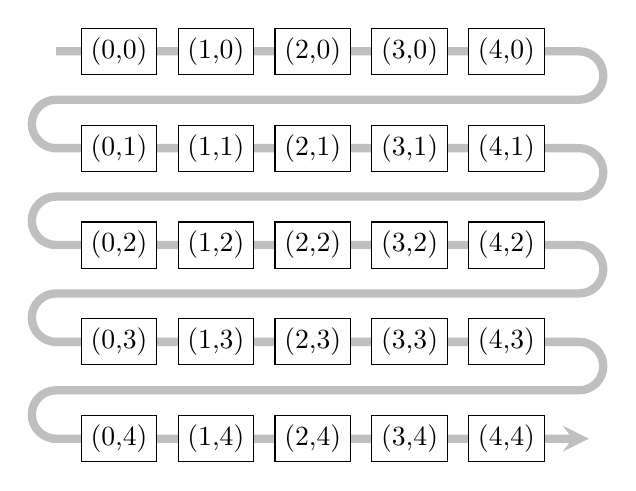
\begin{tikzpicture}[x={(1pt,0)},y={(0,1pt)},scale=0.7]
      \draw[line width=3pt,gray!50,-stealth] (-20,0) 
      \foreach \y in {0,...,3}
      { --  (250,-50*\y) arc(90:-90:12.5)
      --  (-20,-25-50*\y) arc(90:270:12.5)
      -- (-20,-50-50*\y) -- (250, -50-50*\y)
      } --(255,-200);
      \foreach \x in  {0,...,4}
      {\foreach \y in {0,...,4}
       { \node[draw,fill=white] at (12.5+50*\x,-50*\y) (X-\x-\y){(\x,\y)};}
      } 
      \end{tikzpicture}
      \caption{Rappresentazione di una matrice in \textit{row-major order}}
\end{figure}

Nell'ambito della programmazione \texttt{CUDA}, l'accesso agli elementi di
una matrice organizzata secondo il \textit{row-major order} è effettuato
attraverso la seguente formula:
\[
  \texttt{index} = \texttt{row} \times \texttt{width} + \texttt{col}
\]
Questa formula calcola l'indice lineare dell'elemento nella memoria
unidimensionale, dove \texttt{row} rappresenta l'indice della riga,
\texttt{width} la larghezza della matrice, e \texttt{col} l'indice
della colonna.

L'utilizzo del \textit{row-major order} permette un accesso alla memoria
più rapido e prevedibile, essenziale per il parallelismo su \texttt{GPU}.
Gli accessi alla memoria che seguono il pattern naturale della memoria cache
e dei banchi di memoria della \texttt{GPU} riducono i colli di bottiglia
e migliorano il throughput delle operazioni.


\subsection{Gestione dei grid e dei blocchi}
Nella moltiplicazione di matrici tramite \texttt{CUDA}, il dimensionamento
dei blocchi spesso si basa su una tecnica chiamata \textit{tiling}. Questo
approccio permette di ottimizzare l'uso della memoria e migliorare le prestazioni
globali del sistema. Ogni blocco è responsabile del calcolo di un sottoinsieme
della matrice risultante \(C\), e ogni thread all'interno di un blocco calcola
un singolo elemento di \(C\).

Il dimensionamento dei grid e dei blocchi si effettua in modo da dividere
la matrice in ``piastrelle" che possono essere elaborate efficacemente
dai blocchi di thread:

\begin{lstlisting}[language=C]
  // Dimensionamento dei blocchi e dei grid
  dim3 dimGrid(width/TILE_WIDTH, width/TILE_WIDTH, 1);
  dim3 dimBlock(TILE_WIDTH, TILE_WIDTH, 1);
  matMul<<<dimGrid, dimBlock>>>(d_A, d_B, d_C, width);
\end{lstlisting}

Una volta configurati i grid e i blocchi, il kernel \texttt{CUDA} viene
eseguito su ciascun blocco per calcolare i valori corrispondenti nella
matrice \(C\). Il kernel dettagliato è mostrato di seguito:

\begin{lstlisting}[language=C]
  // Definizione del kernel CUDA
  __global__ void matMul(float *A, float *B, float *C, int width) {
    int col = blockIdx.x * blockDim.x + threadIdx.x;
    int row = blockIdx.y * blockDim.y + threadIdx.y;
    float p_val = 0;
    if (row < width && col < width) {
        for (int k = 0; k < width; ++k) {
            p_val += A[row * width + k] * B[k * width + col];
        }
        C[row * width + col] = p_val;
    }
  }
\end{lstlisting}

Questo kernel esegue un ciclo attraverso ogni elemento corrispondente
nelle righe di \(A\) e nelle colonne di \(B\) per accumulare il prodotto
nel valore \(p\_val\), che viene poi assegnato all'elemento corrispondente in \(C\).

\section{Thread \texttt{CUDA}}
Le thread in \texttt{CUDA} sono organizzate in blocchi e griglie, che
forniscono una struttura gerarchica per l'esecuzione parallela. Ogni
thread è identificata da un indice unico all'interno del blocco e della
griglia, che può essere utilizzato per accedere ai dati e coordinare
le operazioni tra le thread.

\section{Modello di Programmazione \texttt{CUDA}}
Il modello di programmazione \texttt{CUDA} consente una scalabilità trasparente attraverso un'assegnazione dinamica dei blocchi di thread e una gestione flessibile delle esecuzioni, adattandosi automaticamente al numero di processori paralleli disponibili.

\subsection{Scalabilità Trasparente nel Modello \texttt{CUDA}}
Nel modello \texttt{CUDA}, l'hardware ha 
la completa libertà di assegnare i blocchi di thread a 
qualsiasi processore in qualsiasi momento, consentendo al kernel 
di scalare su un numero arbitrario di processori paralleli. Questa 
flessibilità è fondamentale per massimizzare l'efficienza di 
esecuzione e le prestazioni del sistema. 

\begin{figure}[H]
  \centering
  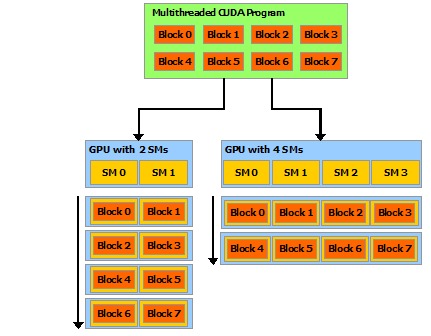
\includegraphics[width=0.7\textwidth]{img/transparent_scalability.png}
\end{figure}

\subsection{Dettagli Tecnici di Scheduling e Gestione dei \texttt{SM}}
I blocchi di thread sono organizzati in griglie di blocchi, e ogni blocco 
può essere eseguito in un ordine indipendente rispetto agli altri. 
La granularità dell'assegnazione dei thread ai multiprocessori 
streaming (\texttt{SM}) varia in base alla generazione del processore:
\begin{itemize}
    \item Gli \texttt{SM Fermi} possono gestire fino a $1536$ thread, 
    con configurazioni come $256$ thread per blocco per $6$ blocchi o $512$ thread per blocco per $3$ blocchi.
    \item Gli \texttt{SM Kepler} possono gestire fino a $2048$ thread, 
    con i thread che vengono eseguiti contemporaneamente.
\end{itemize}
Gli \texttt{SM} mantengono e gestiscono gli identificativi di thread 
e blocco, pianificando l'esecuzione dei thread in modo efficiente.

\subsection{Warps come Unità di Scheduling}
All'interno degli \texttt{SM}, ogni blocco viene eseguito come
warps di $32$ thread, che sono le unità di scheduling. Ad esempio,
se a un \texttt{SM} sono assegnati $3$ blocchi e ogni blocco ha
$256$ thread, il numero totale di warps per \texttt{SM} sarà di
$24$, calcolato come \(256/32 = 8\) warps per blocco moltiplicato 
per $3$ blocchi.

\section{Partizione dei Blocchi di Thread e Controllo del Flusso
in \texttt{CUDA}}
Comprendere come i blocchi di thread sono partizionati e gestiti
all'interno del modello di esecuzione di \texttt{CUDA} è fondamentale
per ottimizzare le prestazioni e garantire un comportamento corretto
dell'applicazione.

\subsection{Partizione dei Blocchi di Thread}
I blocchi di thread in \texttt{CUDA} sono partizionati in warp,
con \texttt{ID} di thread consecutivi e crescenti all'interno di
un warp. Questa partizione è consistente tra le esecuzioni, il
che permette ai programmatori di anticipare e pianificare il
comportamento dei thread all'interno dei warp:
\begin{itemize}
    \item Ogni warp inizia con l'\texttt{ID} di thread 0.
    \item I warp sono strutturati in modo che gli \texttt{ID} di
    thread siano sempre consecutivi, migliorando la prevedibilità
    nel controllo del flusso.
\end{itemize}
Tuttavia, i programmatori non dovrebbero fare affidamento su un
ordine specifico tra i warp a causa delle potenziali dipendenze
tra i thread, che necessitano di una sincronizzazione esplicita
utilizzando \texttt{\_\_syncthreads()} per ottenere risultati di esecuzione corretti.

\subsection{Controllo del Flusso in \texttt{CUDA}}
Il controllo del flusso all'interno di \texttt{CUDA} è soggetto a
problemi di divergenza, dove i thread all'interno di un singolo warp
possono seguire percorsi di esecuzione differenti:
\begin{itemize}
    \item La divergenza si verifica quando i thread in un warp seguono
    percorsi di controllo differenti, che vengono poi serializzati,
    potenzialmente degradando le prestazioni.
    \item Un esempio di divergenza: se \texttt{(threadIdx.x > 2)},
    questa condizione crea due percorsi all'interno del primo warp.
    \item Per minimizzare la divergenza, è consigliabile allineare
    le condizioni di ramificazione con i confini dei warp, ad esempio,
    \texttt{if (threadIdx.x / WARP\_SIZE > 2)}.
\end{itemize}

\subsection{Schedulazione e Esecuzione dei Warp}
La schedulazione dei warp è gestita dai Multiprocessori di Streaming
(\texttt{SM}) con zero sovraccarico:
\begin{itemize}
    \item I warp vengono eseguiti in base alla prontezza degli operandi
    e alle politiche di schedulazione prioritarie.
    \item Questo assicura che tutti i thread in un warp eseguano
    la stessa istruzione simultaneamente quando selezionati, ottimizzando il throughput.
\end{itemize}

\subsection{Considerazioni sulla Granularità dei Blocchi per una
Performance Ottimale}
Scegliere la dimensione giusta del blocco è cruciale per la performance,
specialmente in applicazioni come la moltiplicazione di matrici:
\begin{itemize}
    \item Per una configurazione di blocco $8 \times 8$
    (\textit{$64$ thread per blocco}), un \texttt{SM} può supportare
    fino a $24$ blocchi, ma a causa dei vincoli hardware, spesso solo
    $8$ blocchi possono essere attivi contemporaneamente.
    \item Una configurazione di blocco $16 \times 16$
    (\textit{$256$ thread per blocco}) permette a un \texttt{SM}
    di operare vicino alla piena capacità con fino a $6$ blocchi.
    \item Blocchi più grandi, come $32 \times 32$
    (\textit{$1024$ thread per blocco}), possono superare la
    capacità per \texttt{SM} di alcune versioni di \texttt{CUDA}
    e hardware, riducendo l'efficienza.
\end{itemize}

Ciascuna di queste considerazioni gioca un ruolo significativo nel
determinare quanto efficacemente un programma \texttt{CUDA} può operare, e comprenderle è fondamentale per sfruttare appieno le capacità di \texttt{CUDA}.
